\chapter{Theoretische Grundlagen}
\fancyhfStyleContent{}


\section{Digitale Zwillinge}
\section{Aspektmodelle}
\section{Resource Description Framework (RDF)}

Das Resource Description Framework (RDF) ist ein Modell, das zur Beschreibung von Daten eingesetzt wird \cite[vgl.][]{w3c2014rdf}. Die Datenstruktur formt einen gerichteten Graphen, der sich aus Knoten und Verbindungen (Kanten) zwischen der Knoten zusammensetzt. Ein Ziel von RDF ist, einen Standard schaffen, der emöglicht, beliebige Informationen in maschinenlesbarer Form darzustellen \cite[vgl.][Sektion 2]{w3c2014rdfprimer}.

Zu RDF gehören mehrere Spezifikationen, die beispielsweise das Datenmodell oder eine Syntax zur Beschreibung von Daten festlegen. Das World Wide Web Consortium (W3O) veröffentlicht diese Spezifikationen und viele weitere unter dem Begriff "`Semantic Web"'. Dieser Ausdruck beschreibt die Vision, dass beliebige Daten im Internet bereitgestellt, ausgetauscht und verarbeitet werden können. \cite[vgl.][]{w3c2014semanticweb}

\subsection{Datenmodell}

Ein RDF-Graph setzt sich aus einer beliebig großen Menge sogenannter Triples zusammen. \cite[vgl.][Sektion 3.1]{w3c2014rdfconcepts} Ein einzelnes Triple ist formal gesehen ein 3-Tupel mit folgenden Elementen:
\begin{enumerate}
	\item Das erste Element bezeichnet man als Subjekt. Es repräsentiert den Startknoten, von dem eine Verbindung ausgeht.
	\item Das zweite Element nennt man Prädikat. Es stellt die konkrete Verbindung dar.
	\item Das dritte Element bezeichnet man als Objekt. Dies ist der Endknoten, auf den die Verbindung zeigt. 
\end{enumerate}

Somit sind Subjekt und Objekt immer ein Knoten, das Prädikat ist immer eine Kante.

Es gibt drei Arten von Knoten:
\begin{enumerate}
	\item Als Resource bezeichnet man einen Knoten, der sowohl Ein- als auch Ausgangsknoten besitzen kann und durch einen URI identifiziert. URI sind innerhalb eines Graphen einzigartig und können von Computerprogrammen eingesetzt werden, um einen bestimmten Knoten zu suchen.
	\item Blank Nodes sind Knoten, die Ein- und Ausgangsknoten besitzen können, aber nicht durch einen URI identifiziert sind. Ein Programm kann nicht nach einem Blank Node suchen.
	\item Literale sind Werte wie Ganzzahlen oder Strings und haben keine ausgehenden Kanten.	
\end{enumerate}
Kanten werden immer durch einen URI identifiziert.

In Tabelle \ref{tab:triples} sind Beispiele für Triples zu sehen, die zusammen einen Graphen formen. Die beiden URIs \textless urn:relation\#Anton\textgreater und \textless urn:relation\#Berta\textgreater sind Resourcen. \_:Geburtstag ist eine Blank Node und die Werte "`Anton"', "`Stuttgart"' und "`1980-01-01"'sind Literale.

\begin{table}
	\centering
	\begin{tabular}{c|c|c}
		Subjekt & Prädikat & Objekt \\ \hline
		\textless urn:relation\#Anton\textgreater & \textless urn:relation\#name\textgreater & "'Anton"' \\
		\textless urn:relation\#Anton\textgreater & \textless urn:relation\#hatKind\textgreater & \textless urn:relation\#Berta\textgreater \\
		\textless urn:relation\#Berta\textgreater & \textless urn:relation\#hatVater\textgreater & \textless urn:relation\#Anton\textgreater \\
		\textless urn:relation\#Berta\textgreater & \textless urn:relation\#geboren\textgreater & \_:Geburtstag \\
		\_:Geburtstag & \textless urn:relation\#ort\textgreater & "'Stuttgart"' \\
        \_:Geburtstag & \textless urn:relation\#datum\textgreater & "'1980-01-01"' \\
	\end{tabular}
	\caption{Beispiele für Triples}
	\label{tab:triples}
\end{table}

\begin{figure}
	\centering
	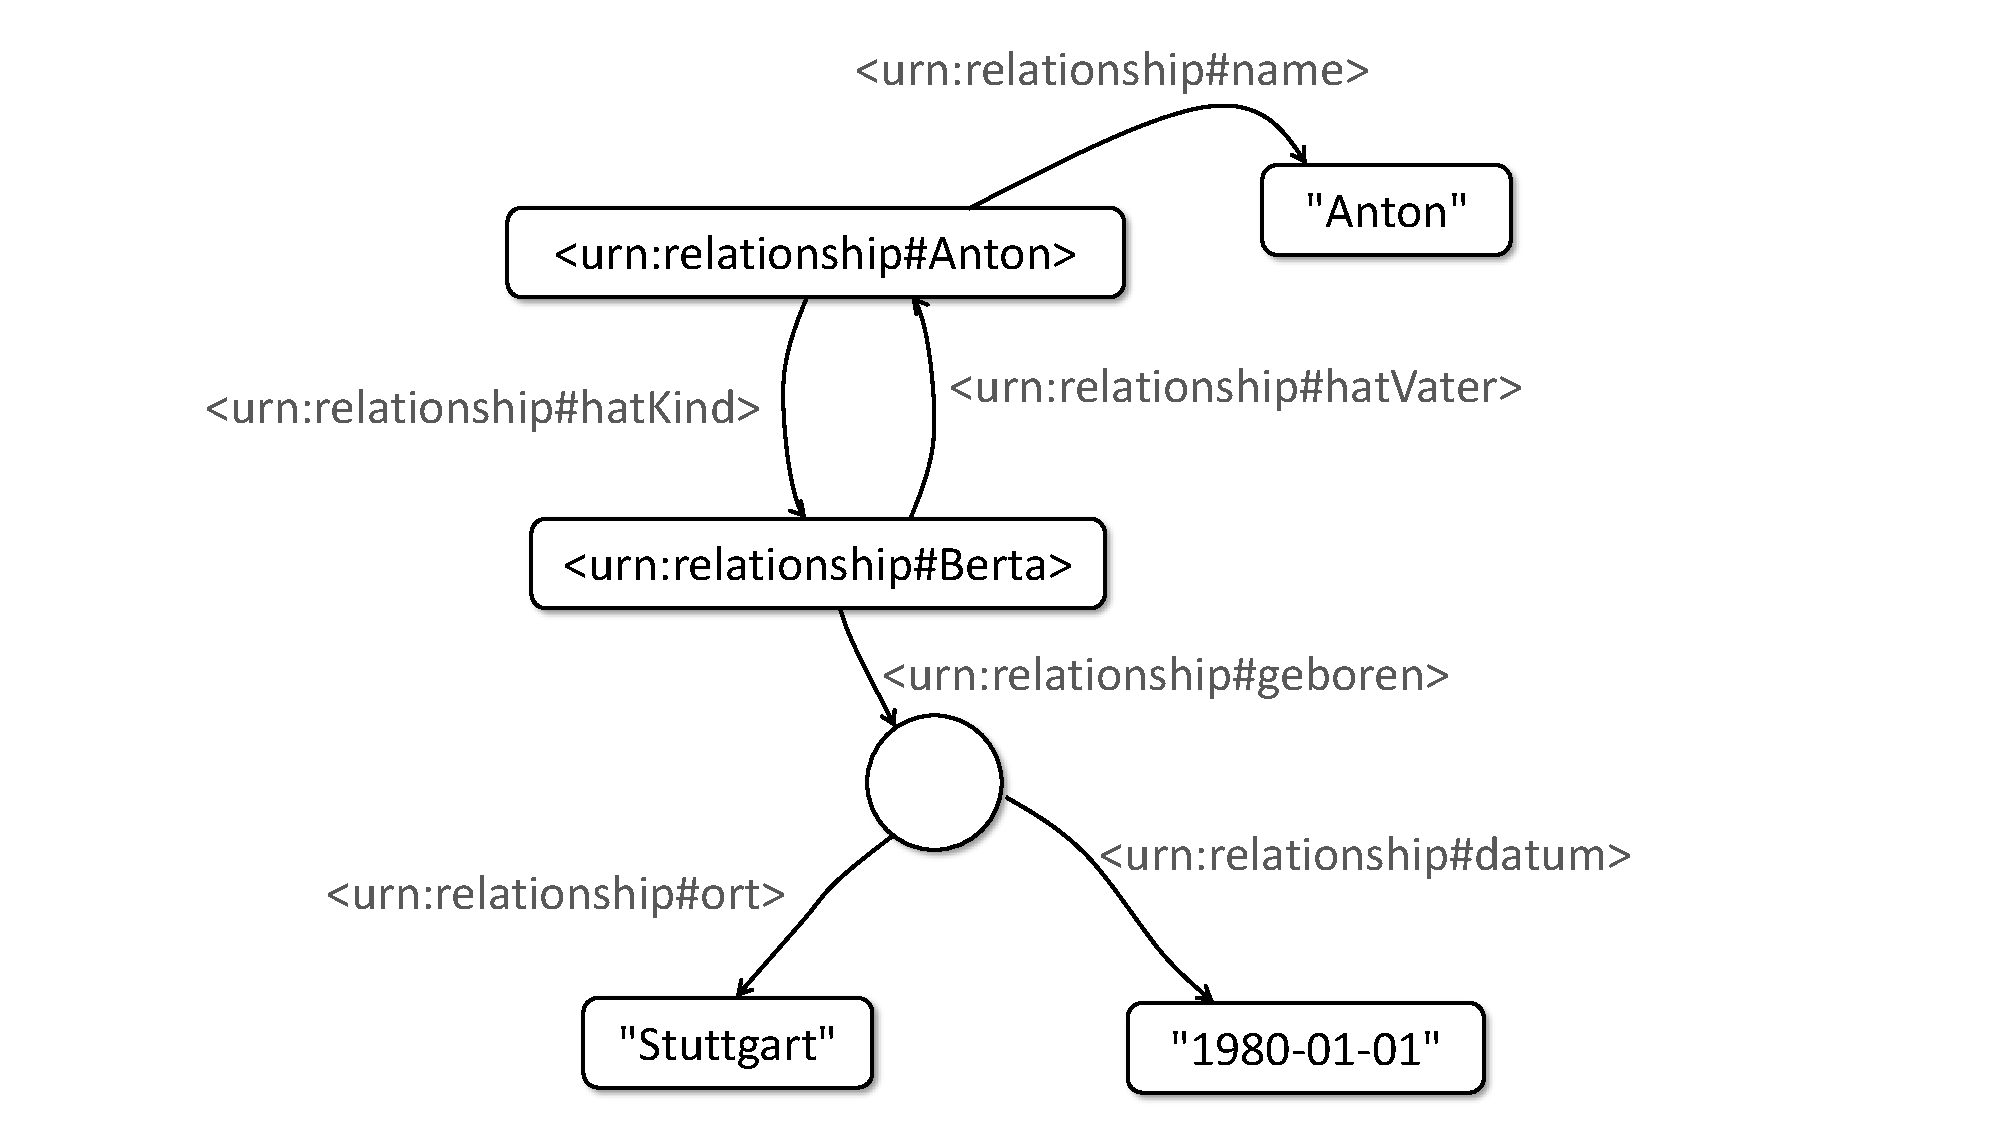
\includegraphics[width=0.7\linewidth]{resources/figures/rdfGraph}
	\caption{}
	\label{fig:rdfgraph}
\end{figure}


\subsection{RDF Syntax}

N-Triples ist eine Syntax, bei der beliebig viele Triples hintereinander aufgelistet werden \cite[vgl.][]{w3c2014ntriples}. Die Grammatik ist in Form von regulären Ausdrücken definiert. Ein Ausschnitt davon ist in den Formeln \ref{eq:ntriple} zu sehen. Jedes n-Triples-Dokument setzt sich demnach aus abwechselnden Triples und Zeilenumbrüchen (EOL, End-Of-Line) zusammen. Ein Triple besteht aus Subjekt, Prädikat und Objekt sowie einem Punkt am Ende. N-Triples-Dateien werden mit der Dateiendung "`.nt"' versehen. Die beispielhaften Triples aus Tabelle \ref{tab:triples} sind in Quellcode \ref{lst:n-triple} dargestellt.
\begin{align}
	\text{ntripleDoc} & ::= \text{triple?}\text{ } (\text{EOL triple})\mbox{*} \text{ EOL?} \label{eq:ntriple}\\
	\text{triple} & ::= \text{subject } \text{predicate } \text{object } \text{"'."'} \nonumber
\end{align}
\listingfile[caption=Beispiel einer N-Triples-Datei, label=lst:n-triple]{resources/codeSnippets/2PureTriples.ttl}

Eine zweite Syntax, mit der RDF-Graphen beschrieben werden können, heißt "`Terse RDF Triple Language"' (TTL) und wird auch als "`Turtle"' bezeichnet  \cite[vgl.][]{w3c2014turtle}. Turtle-Dateien besitzen die Datei-Endung "`.ttl"'.
Die Sprache, die von der TTL-Grammatik beschrieben wird, ist eine Obermenge der N-Triples-Sprache. Das heißt, jede gültige N-Triples-Datei ist auch eine gültige Turtle-Datei. Zusätzlich erlaubt die Turtle-Syntax weitere Schreibweisen, die es ermöglichen, Graphen übersichtlicher und mit weniger Text darzustellen. Durch syntaktische Äquivalenzumformungen lässt sich jede Turtle-Datei wieder auf eine Liste von Triples zurückführen. Somit kann jeder beliebige Graph sowohl mit N-Triples als auch mit Turtle beschrieben werden. Im Folgenden werden einige wichtige Syntax-Merkmale genauer vorgestellt.
\paragraph{Namespaces}

Die URIs in einer Datei beginnen häufig mit dem gleichen Zeichenfolge. Benannte Knoten unterscheiden sich meist nur am letzten Abschnitt des URIs. Namespaces ermögichen, eine abgekürzte Schreibweise für URIs zu verwenden, um die Datei übersichtlicher zu machen. Ein Namespace wird mit dem Schlüsselwort \lstinline|@prefix| festgelegt, wie in Quellcode \ref{lst:ttl-namespace} zu sehen ist.
\listingfile[caption=TTL-Datei mit Namespace, label=lst:ttl-namespace]{resources/codeSnippets/2TriplesNamespace.ttl}

\paragraph{Liste von Prädikaten}
Wenn in einer Turtle-Datei mehrere Triples mit dem gleichen Subjekt vorkommen, können diese Triples zusammengefasst werden. Dazu wird das erste Triple nicht mit einem Punkt, sondern mit einem Semikolon abgeschlossen. In der nächsten Zeile kommen dann nur noch Prädikate und Objekt vor. Das Subjekt wird aus der vorangegangenen Zeile wiederverwendet (siehe Quellcode \ref{lst:ttl-predicate-list}).
\listingfile[caption=TTL-Datei mit einer Liste von Prädikaten, label=lst:ttl-predicate-list]{resources/codeSnippets/2TriplesPredicateList.ttl}

\paragraph{Verschachtelung von Blank Nodes}
Blank Nodes werden häufig eingesetzt, um komplexe Strukturen darzustellen. Im Beispiel setzt sich der Geburtstag aus Ort und Datum zusammen. Blank Nodes werden immer in einem bestimmten Kontext verwendet und verlieren ohne diesen Kontext ihre semantische Bedeutung. Der Knoten \lstinline|_:Geburtstag| beispielsweise ist bedeutungslos, wenn man nicht weiß, dass er zu Berta gehört. Aus diesem Grund ist es sinnvoll, dass der Knoten nicht durch einen URI auffindbar ist. Auf ihn kann nur zugegriffen werden, indem man vom Knoten Berta entlang dem Prädikat \lstinline|rel:geboren| navigiert.

Auch für Blank Nodes gibt es eine Kurzschreibweise. Im Beispiel wird anstatt \lstinline|_:Geburtstag| ein Paar eckiger Klammers \lstinline|[]| geschrieben. Alle Prädikate, die von dem Blank Nodes ausgehen, werden zusammen mit dem Objekt in die eckigen Klammern geschrieben (siehe Quellcode \ref{lst:ttl-blank-node})
\listingfile[caption=TTL-Datei mit verschachtelter Blank Node, label=lst:ttl-blank-node]{resources/codeSnippets/2TriplesBNode.ttl}

\paragraph{RDF-Listen}
Es gibt die Möglichkeit, von einem Knoten mehrere ausgehende Kanten zu spezifizieren, die den gleichen URN haben (siehe Quellcode \ref{lst:ttl-list} oben). Diese Modellierungmöglichkeit kann sehr einfach eingesetzt werden, aber hat den Nachteil dass die Reihenfolge der Objekte nicht spezifiziert ist. Würde man in einem Computerprogramm alle Kinder von Anton in einer Liste sammeln, ist die Reihenfolge der Elemente abhängig von der Implementierung. 

Möchte man eine Liste definieren, bei der die Reihenfolge festgelegt ist, kann man RDF-Listen einsetzen (siehe Quellcode \ref{lst:ttl-list} unten). Bei der Syntax werden runde Klammern eingesetzt. Wenn Die TTL-Datei geparst wird, ist die Liste als Binärbaum dargestellt (siehe \ref{fig:rdflist}). Jeweils ein Ausgang des Knotens zeigt auf ein Listenelement, der andere Ausgang auf den Rest der Liste. Das Ende der Liste wird durch ein spezielles Objekt (rdf:nil) markiert.

\listingfile[caption=Knoten mit mehreren ausgehenden Kanten mit dem gleichen URI, label=lst:ttl-list]{resources/codeSnippets/2TriplesList.ttl}
\begin{figure}
	\centering
	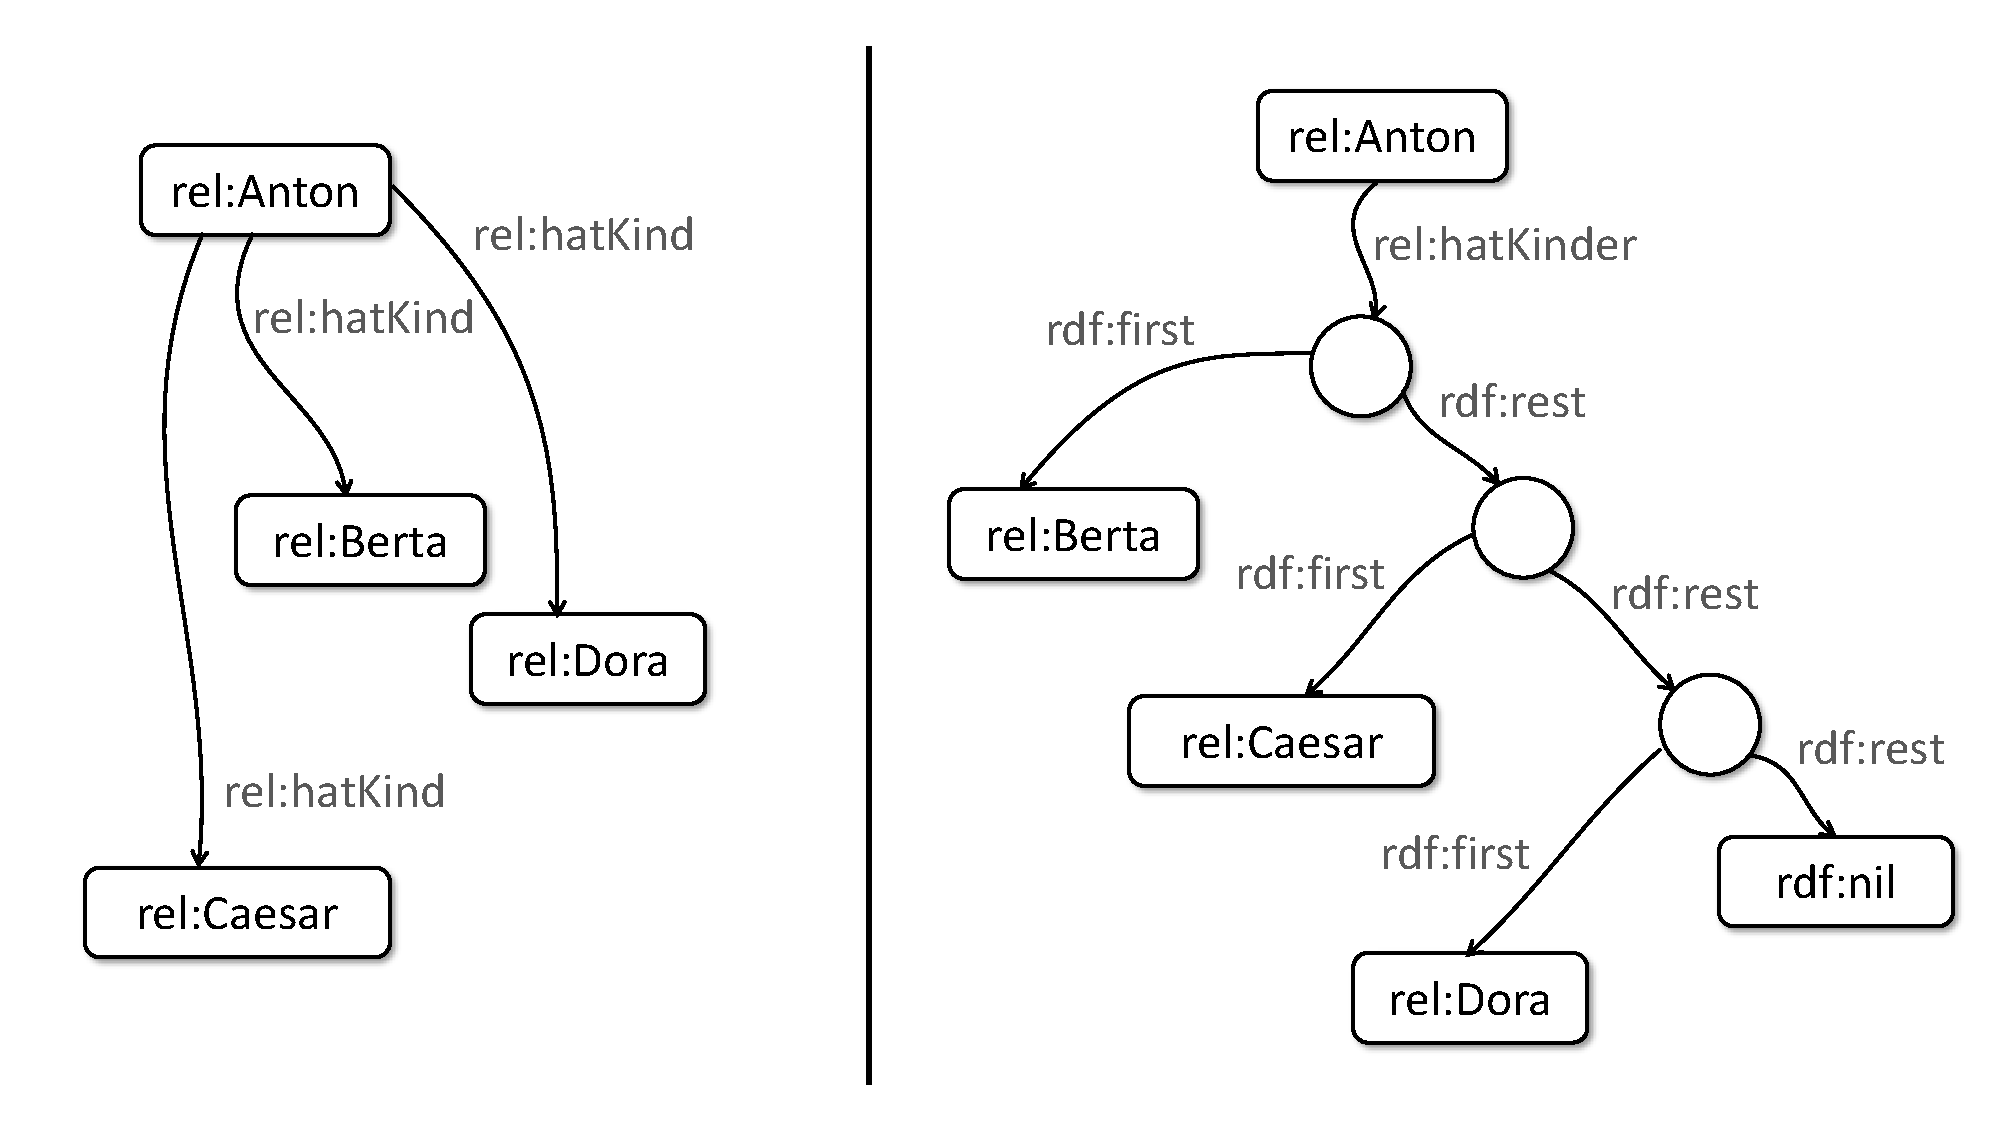
\includegraphics[width=0.7\linewidth]{resources/figures/rdfList}
	\caption[Vergleich von Merhfachverwendung eines Prädikats und RDF-Listen]{Vergleich der beiden Graphen bei mehrfacher Verwendung eines Prädikats (links) und beim Einsatz von von RDF-Listen (rechts).}
	\label{fig:rdflist}
\end{figure}



\section{Software Defined Vehicle}

